\documentclass[10pt]{article}
\usepackage[paperwidth=24in,paperheight=32in,margin=0in]{geometry}
\usepackage{tikz}
\usepackage{graphicx}
\graphicspath{{../}{./}}
\usepackage{amsmath,amssymb}
\usepackage{helvet}
\usepackage{microtype}
\usetikzlibrary{shapes.geometric,arrows.meta,positioning,calc,fit,shadows}
\renewcommand{\familydefault}{\sfdefault}
\pagestyle{empty}
\setlength{\parindent}{0pt}

% ---- Penn State & Technical Color Palette ----
\definecolor{PSNavy}{HTML}{0B2545}        % Deep Penn State Navy
\definecolor{PSBlueMid}{HTML}{1F4E8C}     % Secondary Brand Blue
\definecolor{PSBlueLight}{HTML}{8FB8DE}   % Accent Light Blue
\definecolor{PSBlueIce}{HTML}{E9F1F7}     % Card Header Ice Tint
\definecolor{PSGold}{HTML}{D49B28}        % Warm Accent Gold
\definecolor{BoxNavy}{HTML}{13315C}       % Box Header Navy
\definecolor{DarkText}{HTML}{1A1A1A}      % Crisp Body Text
\definecolor{MutedGray}{HTML}{555555}     % Secondary Text
\definecolor{CardBg}{HTML}{FFFFFF}        % Pure White Card Background
\definecolor{CardBorder}{HTML}{C5D4E3}    % Soft Card Outline
\definecolor{BadgeBg}{HTML}{0B2545}       % Pill Badge Navy
\definecolor{BadgeText}{HTML}{FFFFFF}     % Pill Badge White
\definecolor{HighlightBg}{HTML}{F0F5FA}   % Bullet Highlight Container

% ---- Reusable Card Styling Macro ----
% usage: \ModernCard{x}{y}{w}{h}{Title}{CategoryBadge}
\newcommand{\ModernCardHeader}[6]{%
  \pgfmathsetmacro{\cx}{#1}
  \pgfmathsetmacro{\cy}{#2}
  \pgfmathsetmacro{\cw}{#3}
  \pgfmathsetmacro{\ch}{#4}
  \pgfmathsetmacro{\hdrH}{1.3}
  % Card background & subtle shadow/border
  \draw[CardBorder, line width=1.2pt, fill=CardBg, rounded corners=7pt]
        (\cx,\cy) rectangle (\cx+\cw,\cy+\ch);
  % Top banner header strip
  \fill[PSNavy, rounded corners=7pt] (\cx,\cy+\ch-\hdrH) rectangle (\cx+\cw,\cy+\ch);
  \fill[PSNavy] (\cx,\cy+\ch-\hdrH) rectangle (\cx+\cw,\cy+\ch-\hdrH/2);
  % Header accent line (PSGold)
  \fill[PSGold] (\cx,\cy+\ch-\hdrH-0.08) rectangle (\cx+\cw,\cy+\ch-\hdrH);
  % Category badge on top-right of header
  \node[anchor=east, fill=PSBlueMid, rounded corners=3pt, inner sep=3pt, text=white]
        at (\cx+\cw-0.4, \cy+\ch-\hdrH/2)
        {\bfseries\fontsize{8.5}{10}\selectfont \uppercase{#6}};
  % Card Title (left-aligned)
  \node[anchor=west, text=white] at (\cx+0.5, \cy+\ch-\hdrH/2)
       {\bfseries\fontsize{14}{16}\selectfont #5};
}

\begin{document}

% ============================================================
% 1. TOP HEADER BANNER (Full 24" Width)
% ============================================================
\begin{tikzpicture}[remember picture, overlay, x=1in, y=1in]
  \begin{scope}[shift={(current page.north west)}]
    % Crisp white title background matching logo backgrounds
    \fill[white] (0,0) rectangle (24,-3.8);
    % Top navy & gold accent lines
    \fill[PSNavy] (0,0) rectangle (24,-0.09);
    \fill[PSGold] (0,-0.09) rectangle (24,-0.13);
    % Bottom gold & navy accent lines
    \fill[PSGold] (0,-3.67) rectangle (24,-3.71);
    \fill[PSNavy] (0,-3.71) rectangle (24,-3.80);

    % Penn State Logo (Left - sitting cleanly on white)
    \node[anchor=west] at (0.8, -1.90) {%
      
\includegraphics[height=1.35in, keepaspectratio]{images/PSULogo_hires.png}%
    };

    % Los Alamos National Laboratory Logo (Right - sitting cleanly on white)
    \node[anchor=east] at (23.2, -1.90) {%
      
\includegraphics[height=1.25in, keepaspectratio]{images/LANLLogo.png}%
    };

    % Center Title, Subtitle, Authors, Affiliation
    \node[align=center, text width=14.6in] at (12.0, -1.90) {%
      {\bfseries\fontsize{29}{34}\selectfont\color{PSNavy} High-Throughput Dynamic Material Characterization}\\[0.30em]
      {\bfseries\fontsize{17}{21}\selectfont\color{PSBlueMid} Synergistic Experimental \& Digital Twin Framework for Rate-Dependent Model Discovery}\\[0.45em]
      {\bfseries\fontsize{13.5}{16}\selectfont\color{PSNavy} Zachary Salas$^1$ \quad$\vert$\quad Jeremy Croom$^1$ \quad$\vert$\quad Reuben H. Kraft, Ph.D.$^1$}\\[0.28em]
      {\fontsize{10.5}{13}\selectfont\color{MutedGray} $^1$Department of Mechanical Engineering, The Pennsylvania State University, University Park, PA}
    };
  \end{scope}
\end{tikzpicture}


% ============================================================
% 2. MAIN POSTER CONTENT CANVAS (57 cm x 68 cm)
% ============================================================
\begin{tikzpicture}[remember picture, overlay, x=1cm, y=1cm]
\path (current page.south west) ++(2.0, 1.8) coordinate (canvasorigin);
\begin{scope}[shift={(canvasorigin)}]

% ============================================================
% ROW 1 (y = 46.4 to 68.4 cm, h = 22.0 cm):
% Left: Miniature Kolsky Bar Setup | Right: Abaqus Digital Twin
% ============================================================

% --- CARD 1: Miniature Kolsky Bar Apparatus ---
\ModernCardHeader{0}{46.4}{27.5}{22.0}{Miniature Kolsky Bar Apparatus ($\varnothing 3.17\text{ mm}$)}{Experimental Apparatus}

% Image of Kolsky apparatus + specimen pulse vectors (PSU Mini bar only)
\node[anchor=north west] at (0.6, 66.8) {%
  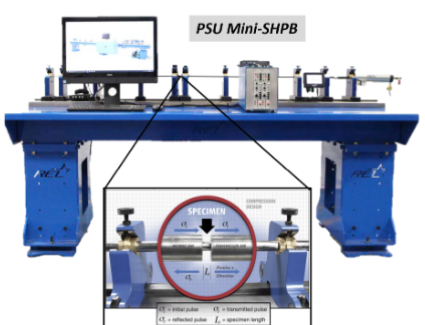
\includegraphics[width=13.4cm, height=10.0cm, keepaspectratio]{images/PSU_MiniKolskyBar_system.png}%
};

% Specifications Card to the right of PSU Mini Bar photo
\fill[PSBlueIce!80, rounded corners=5pt, draw=PSBlueMid!40, line width=0.8pt] (14.3, 56.4) rectangle (27.0, 66.8);
\fill[PSBlueMid, rounded corners=4pt] (14.3, 65.8) rectangle (27.0, 66.8);
\node[anchor=center, text=white] at (20.65, 66.3) {\bfseries\fontsize{8.5}{10}\selectfont HARDWARE ARCHITECTURE};
\node[anchor=north west, text width=12.2cm, align=left] at (14.6, 65.4) {%
  \fontsize{8.2}{11.2}\selectfont
  \textbf{Bar Material:} C350 Maraging Steel\\[0.18em]
  \textbf{Bar Diameter:} $\varnothing 3.17\,\text{mm}$ ($1/8^{\prime\prime}$ OD)\\[0.18em]
  \textbf{Bar Lengths:} Incident $1.0\,\text{m}$, Trans. $1.0\,\text{m}$\\[0.18em]
  \textbf{Wave Speed:} $C_0 \approx 4960\,\text{m/s}$\\[0.18em]
  \textbf{Striker Range:} $L_s = 200\,\text{mm}$, $V_0 \le 30\,\text{m/s}$\\[0.18em]
  \textbf{Pulse Duration:} $T_p \approx 78\,\mu\text{s}$\\[0.18em]
  \textbf{Gauges:} Semiconductor ($10\,\text{MHz}$ DAQ)\\[0.18em]
  \textbf{Max Strain Rate:} $\dot{\varepsilon}_{\max} \sim 1.2 \times 10^4\,\text{s}^{-1}$
};

% Text Box for Card 1
\node[anchor=north west, text width=26.1cm, align=left] at (0.7, 55.8) {%
  \fontsize{10.2}{14.4}\selectfont
  \begin{itemize}\setlength{\itemsep}{0.28em}\setlength{\leftmargin}{1.0em}
    \item \textbf{Ultra-Small Diameter Architecture:} Precision $\varnothing 3.17\,\text{mm}$ C350 maraging steel bar system specifically engineered for sub-scale testing of advanced composites, ductile metals (OFHC copper), and transparent polymers (PMMA).
    \item \textbf{Extreme Dynamic Strain Rate Regime:} Achieves dynamic strain rates from $\dot{\varepsilon} \sim 10^3\text{ to }1.2 \times 10^4\,\text{s}^{-1}$ under strictly verified 1D wave propagation with minimal Pochhammer-Chree dispersion.
    \item \textbf{High-Frequency Diagnostics:} Instrumented with high-bandwidth semiconductor strain gauges at bar midpoints; isolates incident ($\sigma_i$), reflected ($\sigma_r$), and transmitted ($\sigma_t$) stress waves digitized at $10\,\text{MHz}$.
    \item \textbf{High-Throughput Testing Protocol:} Modular alignment guides and precision collets enable rapid shot cycles ($>10\text{ shots/hr}$), providing dense empirical datasets for statistical uncertainty bounds.
  \end{itemize}
};


% --- CARD 2: Abaqus/Explicit Digital Twin ---
\ModernCardHeader{29.5}{46.4}{27.5}{22.0}{Abaqus/Explicit Digital Twin Modeling}{Computational Twin}

% Upper Part: Full Bar Assembly FE schematic + Zoom
\node[anchor=north] at (43.25, 66.8) {%
  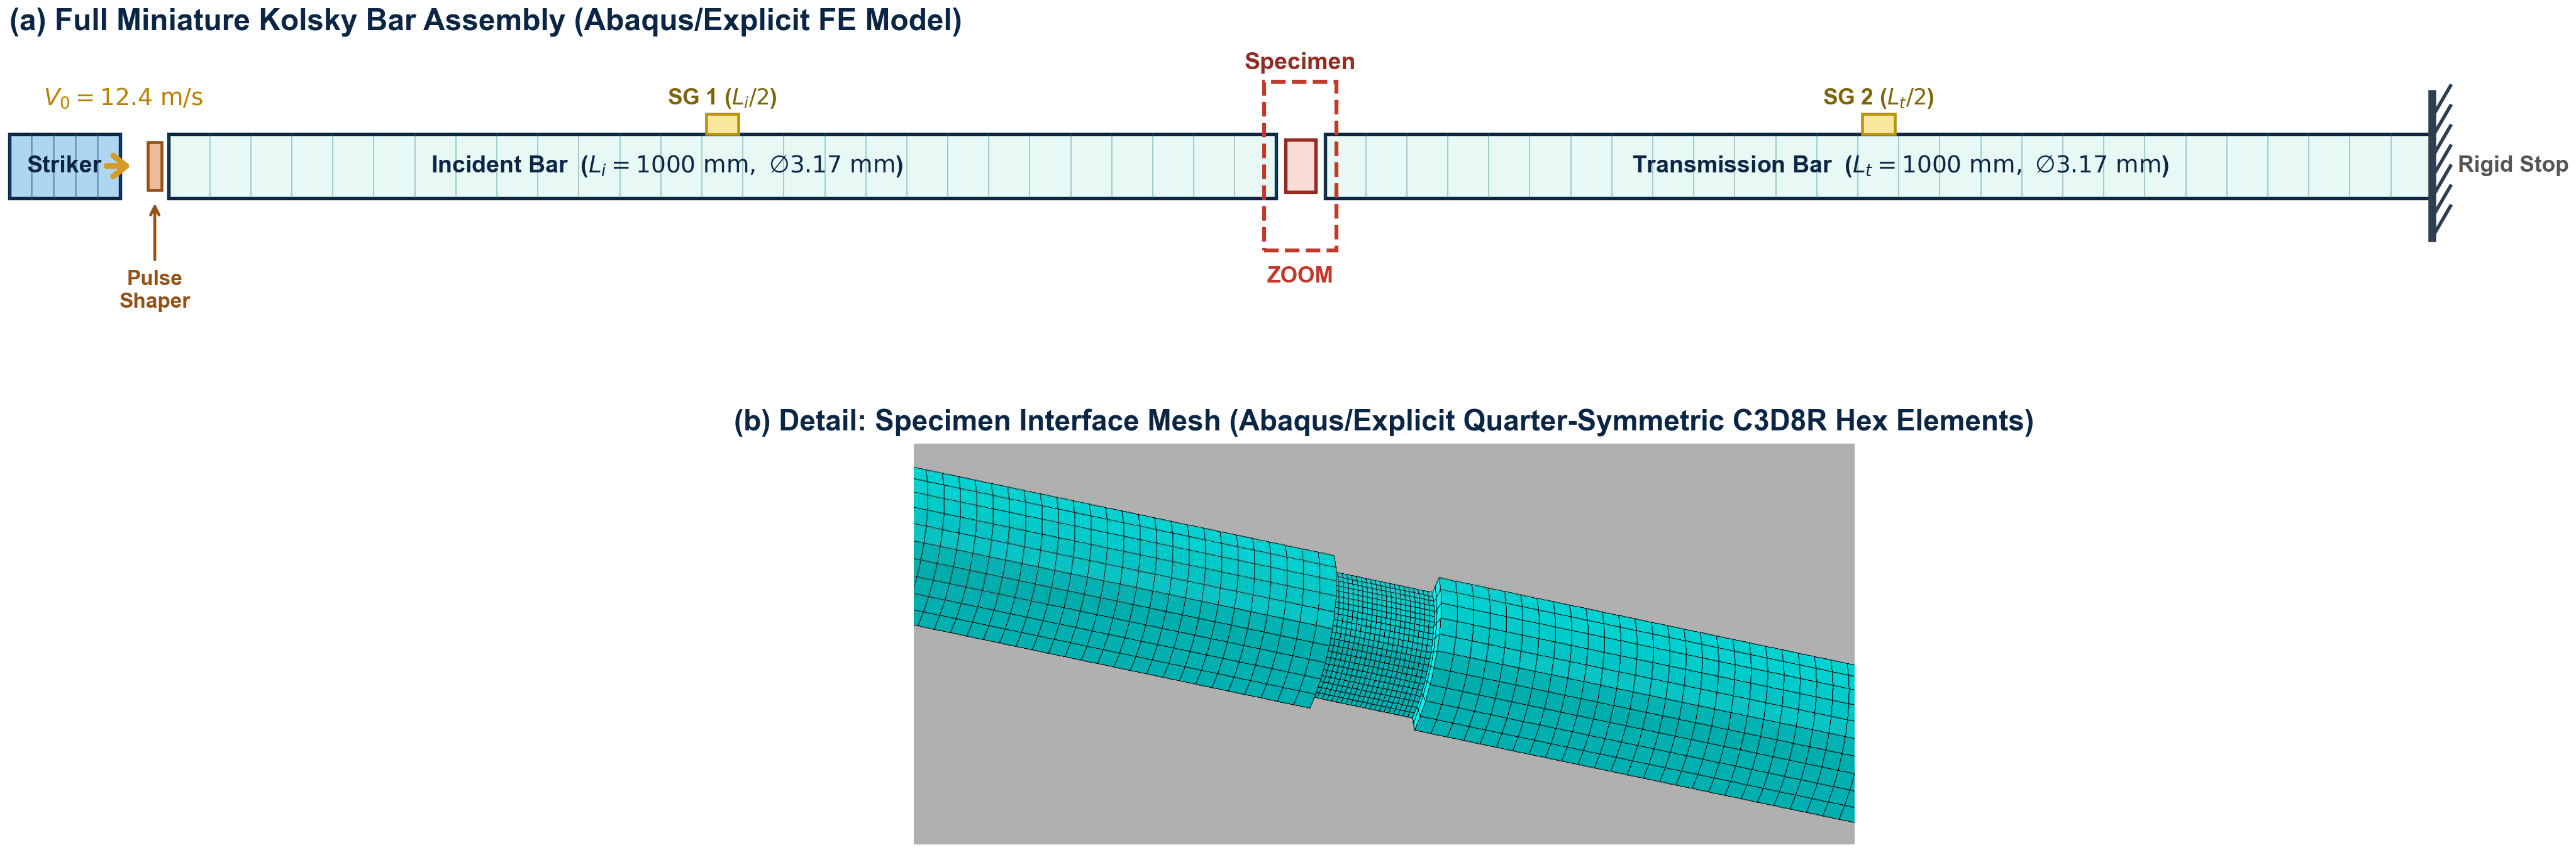
\includegraphics[width=26.2cm, height=7.8cm, keepaspectratio]{images/digital_twin_full_and_zoom.png}%
};

% Digital Twin Core Bullets
\node[anchor=north west, text width=26.1cm, align=left] at (30.2, 59.2) {%
  \fontsize{9.6}{13.2}\selectfont
  \begin{itemize}\setlength{\itemsep}{0.18em}\setlength{\leftmargin}{1.0em}
    \item \textbf{Multi-Symmetry FE Formulations:} 3D quarter- and full-symmetry models constructed in Abaqus/Explicit with C3D8R hex elements for dispersive wave propagation, striker impact, and platen boundary condition verification.
    \item \textbf{Pre-Shot Waveform Optimization:} Virtual striker velocity and boundary impedance sweeps eliminate trial-and-error testing and maximize constant-strain-rate deformation duration.
  \end{itemize}
};

% Lower Part: Dedicated Subsection Container for Innovative Pulse Shaping
\fill[PSBlueIce!60, rounded corners=5pt, draw=PSBlueMid!40, line width=0.8pt] (29.9, 46.8) rectangle (56.6, 55.4);
\fill[PSNavy, rounded corners=4pt] (29.9, 54.4) rectangle (56.6, 55.4);
\node[anchor=west, text=white] at (30.3, 54.9) {\bfseries\fontsize{9.2}{11}\selectfont Innovative Pulse Shaping for Tailored Response};
\node[anchor=east, fill=PSGold, rounded corners=2pt, inner sep=2pt, text=black] at (56.3, 54.9) {\bfseries\fontsize{7.2}{8.5}\selectfont TAILORED WAVEFORMS};

% Subsection Composite Graphic (AM Micro-Lattice + Dynamic Upsetting + Tailored Pulse)
\node[anchor=north] at (43.25, 54.2) {%
  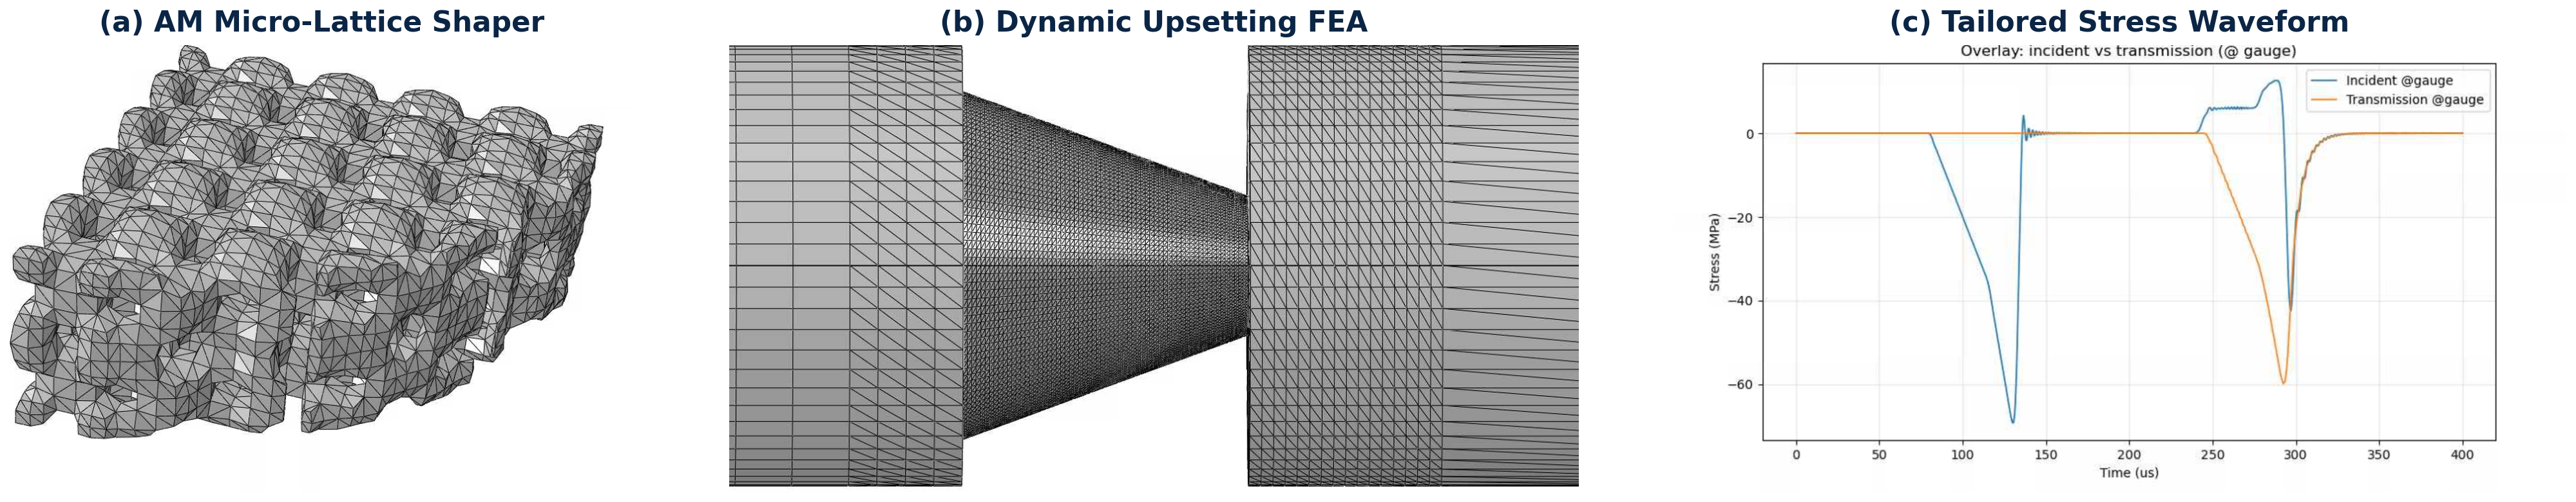
\includegraphics[width=26.0cm, height=4.2cm, keepaspectratio]{images/pulse_shaping_tailored_response.png}%
};

% Subsection Bullets
\node[anchor=north west, text width=26.1cm, align=left] at (30.2, 49.8) {%
  \fontsize{9.4}{12.8}\selectfont
  \begin{itemize}\setlength{\itemsep}{0.18em}\setlength{\leftmargin}{1.0em}
    \item \textbf{AM Micro-Architected Shapers:} Additively manufactured micro-lattices (nTopology/Abaqus) engineered to eliminate high-frequency Pochhammer-Chree wave dispersion and stress spikes.
    \item \textbf{Constant Strain-Rate (CSR) Control:} Programmable rise times dynamically tailor the incident pulse to ensure force equilibrium and constant $\dot{\varepsilon}$ deformation across soft and hard materials.
  \end{itemize}
};


% ============================================================
% WORKFLOW RIBBON (y = 41.5 to 45.0 cm, h = 3.5 cm):
% 4-Step Closed-Loop Digital-Experimental Process Pipeline
% ============================================================
\fill[PSBlueIce, rounded corners=6pt, draw=PSBlueMid!40, line width=1pt] (0, 41.5) rectangle (57.0, 45.0);

% Step 1 Box
\fill[PSNavy, rounded corners=4pt] (0.4, 41.8) rectangle (13.6, 44.7);
\node[white, align=center, text width=12.8cm] at (7.0, 43.25) {%
  {\bfseries\fontsize{11}{12}\selectfont 1. Virtual Pulse Shaping}\\[0.15em]
  {\fontsize{8.5}{10}\selectfont\color{PSBlueLight} Abaqus sweeps shaper geometry \& velocity}%
};

% Arrow 1 -> 2
\node[text=PSGold] at (14.2, 43.25) {\fontsize{16}{16}\selectfont $\boldsymbol{\blacktriangleright}$};

% Step 2 Box
\fill[PSBlueMid, rounded corners=4pt] (14.8, 41.8) rectangle (28.0, 44.7);
\node[white, align=center, text width=12.8cm] at (21.4, 43.25) {%
  {\bfseries\fontsize{11}{12}\selectfont 2. Specimen \& Shaper Prep}\\[0.15em]
  {\fontsize{8.5}{10}\selectfont\color{white!85} Wire-EDM precision fabrication \& alignment}%
};

% Arrow 2 -> 3
\node[text=PSGold] at (28.6, 43.25) {\fontsize{16}{16}\selectfont $\boldsymbol{\blacktriangleright}$};

% Step 3 Box
\fill[PSNavy, rounded corners=4pt] (29.2, 41.8) rectangle (42.4, 44.7);
\node[white, align=center, text width=12.8cm] at (35.8, 43.25) {%
  {\bfseries\fontsize{11}{12}\selectfont 3. Dynamic Mini-SHPB Run}\\[0.15em]
  {\fontsize{8.5}{10}\selectfont\color{PSBlueLight} 10 MHz strain acquisition + Nova S20 video}%
};

% Arrow 3 -> 4
\node[text=PSGold] at (43.0, 43.25) {\fontsize{16}{16}\selectfont $\boldsymbol{\blacktriangleright}$};

% Step 4 Box
\fill[PSBlueMid, rounded corners=4pt] (43.6, 41.8) rectangle (56.6, 44.7);
\node[white, align=center, text width=12.6cm] at (50.1, 43.25) {%
  {\bfseries\fontsize{11}{12}\selectfont 4. Model Calibration}\\[0.15em]
  {\fontsize{8.5}{10}\selectfont\color{white!85} Extract $\sigma$-$\varepsilon$ curves \& refine digital twin}%
};


% ============================================================
% ROW 2 (y = 20.8 to 40.2 cm, h = 19.4 cm):
% Left: Waveform Alignment & Validation | Right: High-Speed NOVA S20 Filmstrip
% ============================================================

% --- CARD 3: Dynamic Wave Alignment & Equilibrium ---
\ModernCardHeader{0}{20.8}{27.5}{19.4}{Dynamic Wave Alignment \& Validation}{Wave Propagation}

% Stacked Waveform Plots
\node[anchor=north] at (13.75, 39.1) {%
  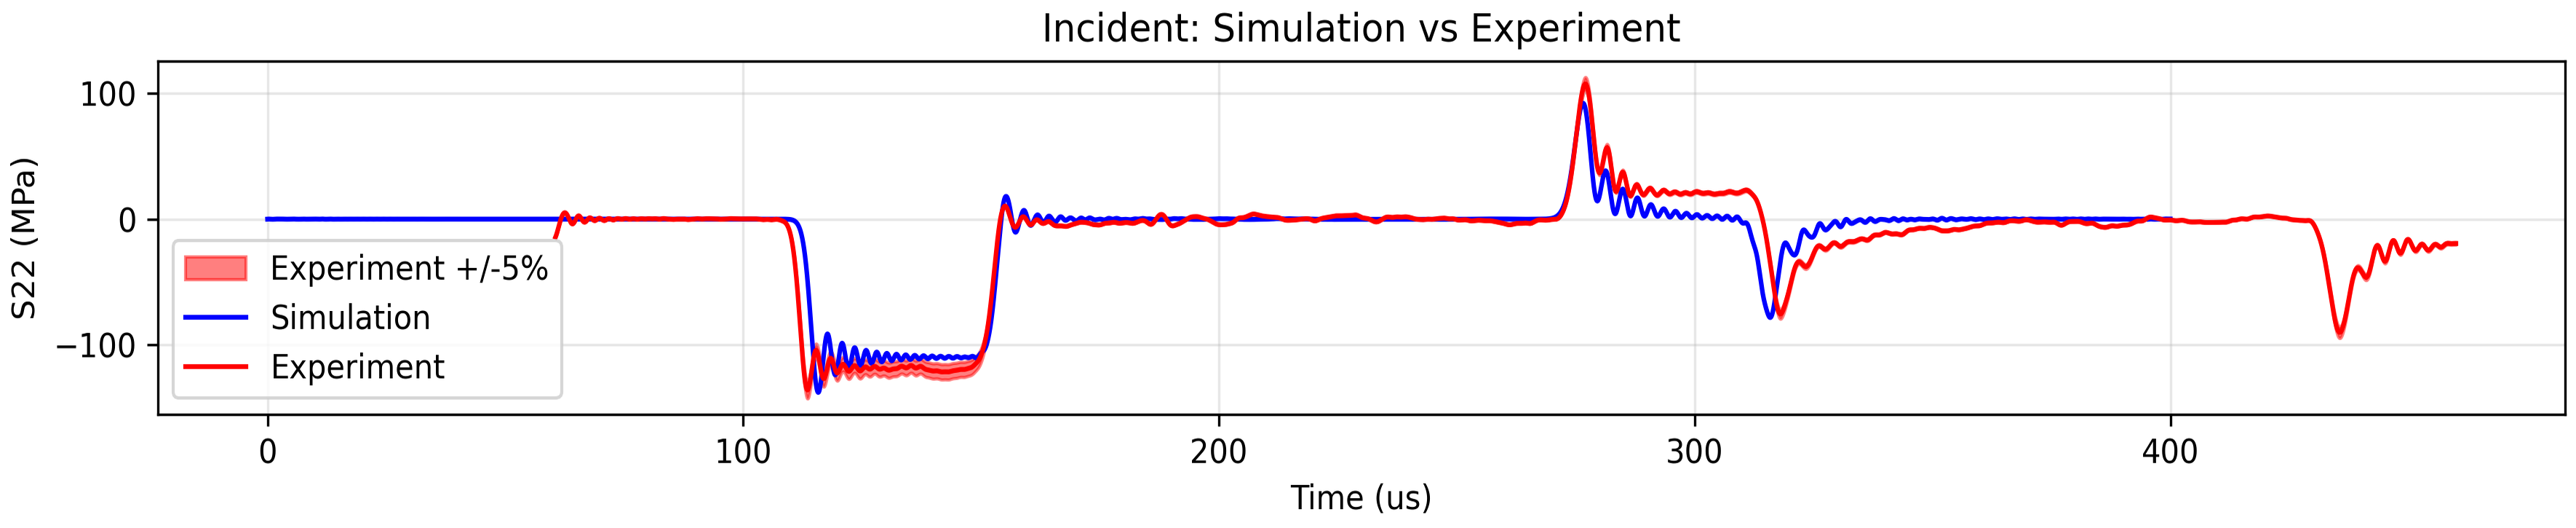
\includegraphics[width=26.3cm, height=4.1cm, keepaspectratio]{images/incidentcomp.png}%
};
\node[anchor=north] at (13.75, 34.8) {%
  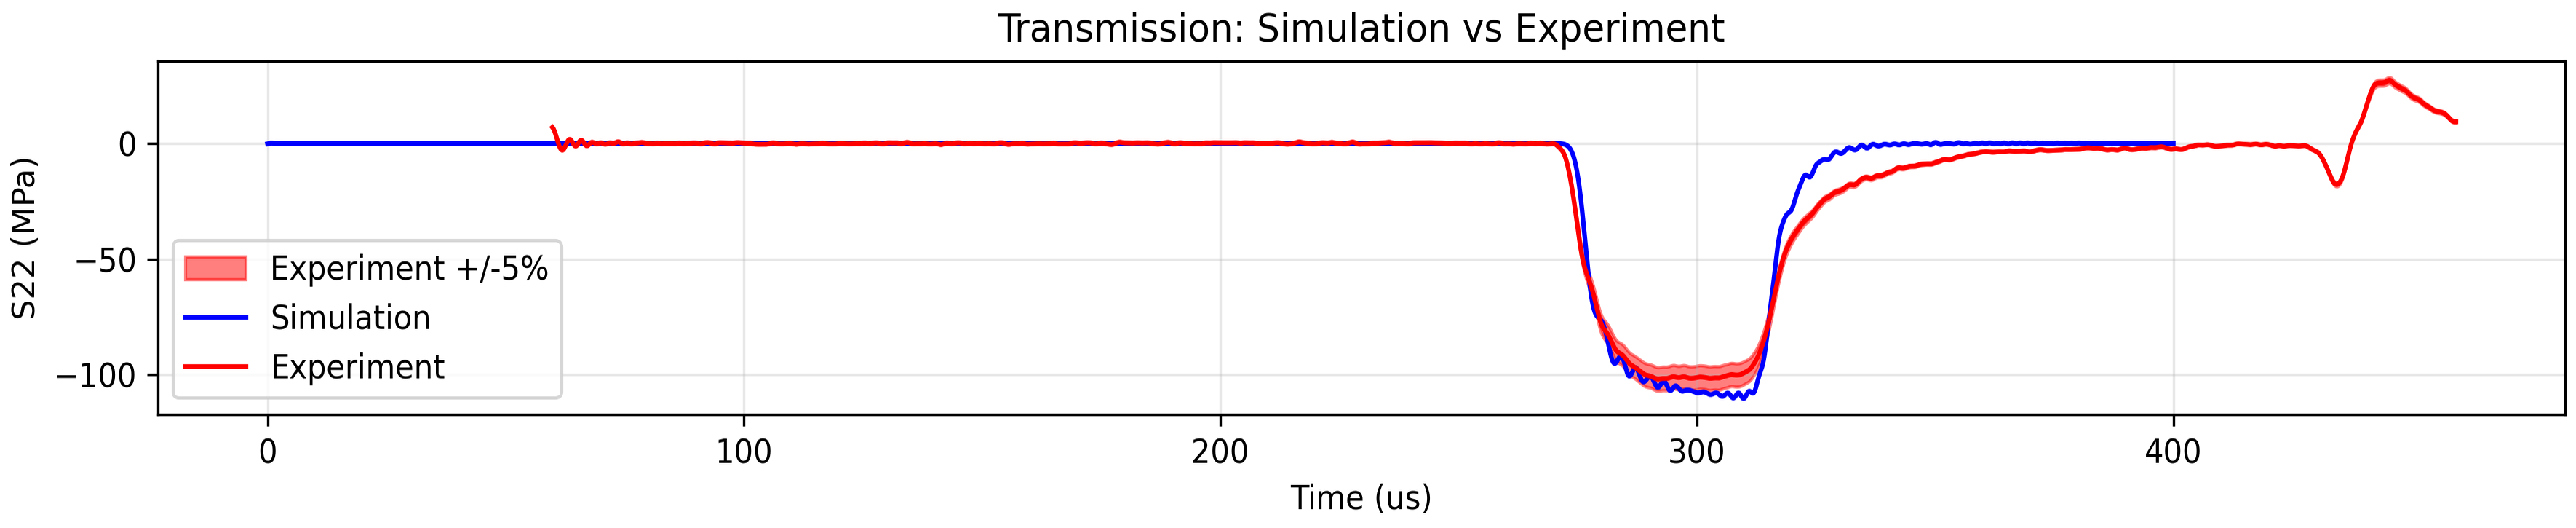
\includegraphics[width=26.3cm, height=4.1cm, keepaspectratio]{images/transmissioncomp.png}%
};

% Text Box for Card 3
\node[anchor=north west, text width=26.1cm, align=left] at (0.7, 30.5) {%
  \fontsize{10.2}{14.5}\selectfont
  \begin{itemize}\setlength{\itemsep}{0.28em}\setlength{\leftmargin}{1.0em}
    \item \textbf{Dispersion-Corrected Voltage Signals:} Incident and transmitted pulses captured at $10\,\text{MHz}$ sampling frequency; wave profiles time-shifted to specimen contact interface.
    \item \textbf{Digital Twin Predictive Accuracy:} Tight overlay between finite element simulation predictions and experimental bridge voltages across the primary pulse duration.
    \item \textbf{Dynamic Force Equilibrium:} Verified across incident and transmission bar platens ($P_1(t) \approx P_2(t)$), ensuring homogeneous stress distribution throughout deformation.
    \item \textbf{Model Refinement Feedback:} Waveform discrepancies directly guide the identification of rate-dependent strain hardening and thermal softening parameters.
  \end{itemize}
};


% --- CARD 4: High-Speed NOVA S20 Imaging ---
\ModernCardHeader{29.5}{20.8}{27.5}{19.4}{Photron FASTCAM Nova S20 High-Speed Video}{Optical Diagnostics}

% Camera Setup Photo (Left)
\draw[CardBorder, fill=black!5, line width=0.8pt, rounded corners=4pt] (30.1, 33.6) rectangle (37.5, 38.6);
\node[inner sep=0pt] at (33.8, 36.1) {%
  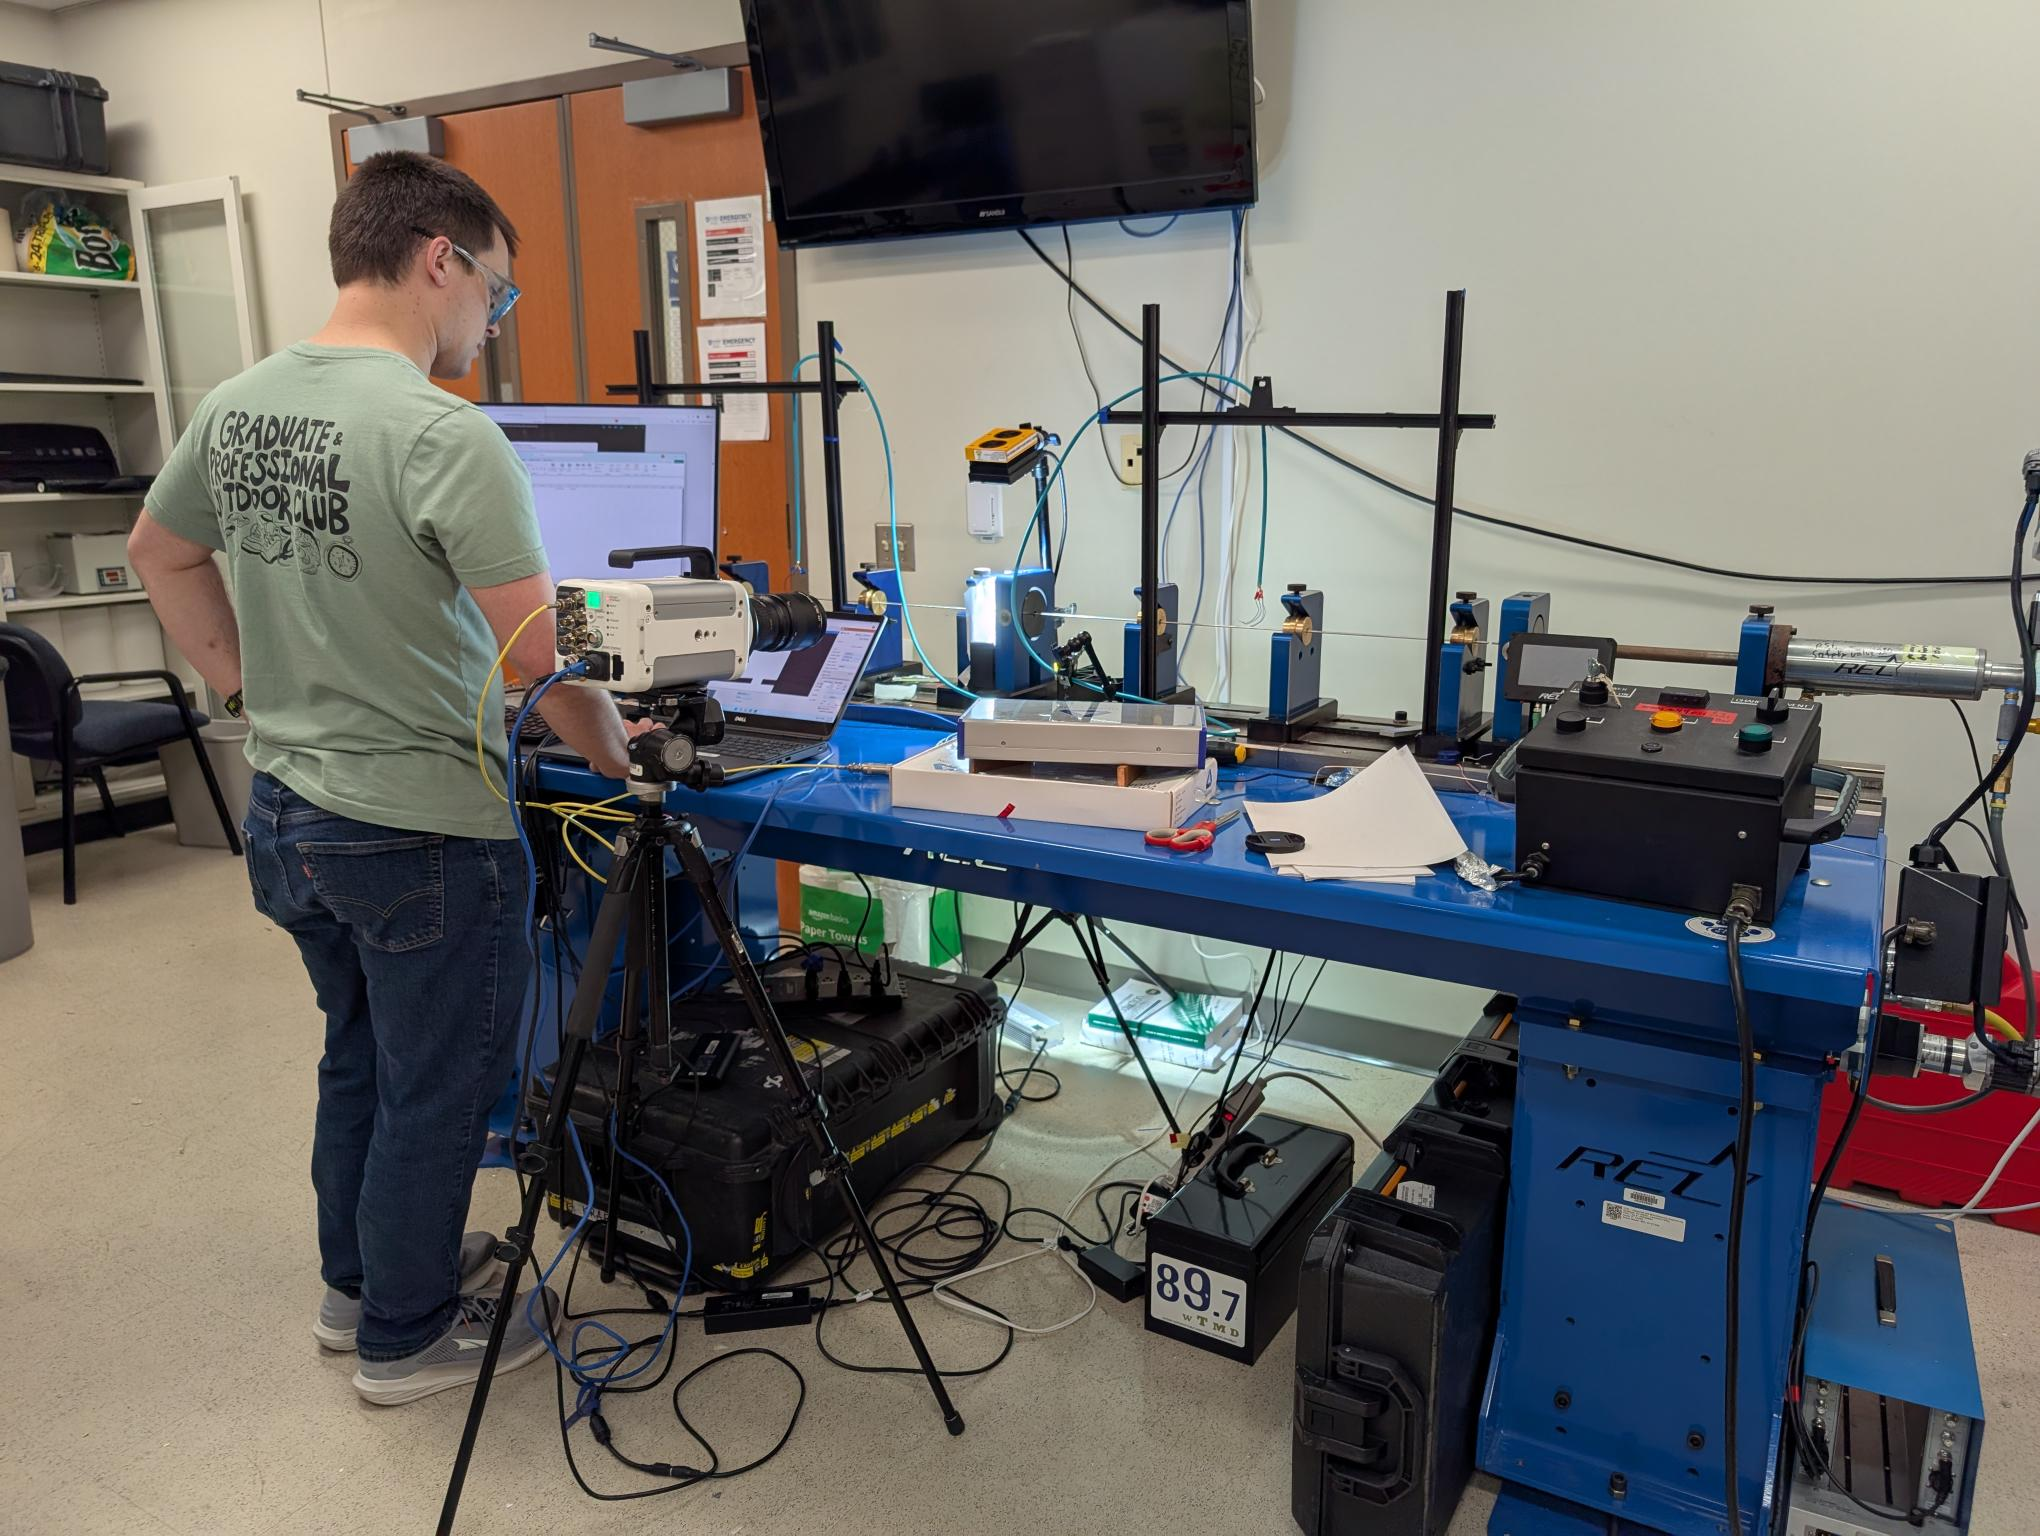
\includegraphics[width=7.2cm, height=4.8cm, keepaspectratio]{images/camera_setup.jpg}%
};
\node[anchor=south, fill=PSNavy!95, text=white, rounded corners=2pt, inner sep=2pt] at (33.8, 33.75) {%
  \bfseries\fontsize{7.5}{9}\selectfont FASTCAM Nova S20 Rig%
};

% Text beside camera setup photo (Right)
\node[anchor=north west, text width=18.4cm, inner sep=0pt, align=left] at (38.2, 38.6) {%
  \fontsize{9.8}{13.4}\selectfont
  \textbf{Optical Configuration \& Synchronization:}\\[0.25em]
  The Photron FASTCAM Nova S20 is coupled with macro-telephoto optics and high-intensity LED matrix illumination, triggered synchronously with the incident bar strain bridge.
  \begin{itemize}\setlength{\itemsep}{0.22em}\setlength{\leftmargin}{0.9em}
    \item \textbf{Framing Rates:} $100,000\text{ to }200,000\,\text{fps}$ with sub-$\mu\text{s}$ exposure to freeze dynamic wave motion.
    \item \textbf{Alignment Verification:} Real-time visualization guarantees coaxial platen impact without bar bending or eccentric loading.
  \end{itemize}
};

% 5-Frame Time-Lapse Filmstrip Container (Centered inside Card 4)
\fill[PSNavy!95, rounded corners=4pt] (30.1, 28.8) rectangle (56.4, 33.0);

% Title strip
\node[anchor=west, text=white] at (30.4, 32.65) {%
  \bfseries\fontsize{8.5}{10}\selectfont High-Speed Dynamic Compression Sequence ($\dot{\varepsilon} \sim 4000\,\text{s}^{-1}$ OFHC Copper on $\varnothing 3.17\,\text{mm}$ C350 Bars)%
};

% 5 Frames placed with exact coordinates: width=5.0cm, gap=0.2cm, height=3.25cm
% Frame 1
\draw[white!40, fill=black, line width=0.6pt] (30.35, 29.0) rectangle (35.35, 32.25);
\node[inner sep=0pt] at (32.85, 30.625) {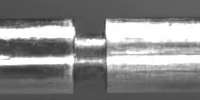
\includegraphics[width=4.9cm, height=3.15cm]{images/copper_f1.png}};
\node[anchor=south west, fill=PSGold, text=black, rounded corners=1.5pt, inner sep=1.2pt] at (30.45, 29.08) {\bfseries\fontsize{6.5}{7.5}\selectfont $0.0\,\mu\text{s}$};
\node[anchor=south east, fill=black!75, text=white, rounded corners=1.5pt, inner sep=1.2pt] at (35.25, 29.08) {\fontsize{6.2}{7.2}\selectfont Initial};

% Frame 2
\draw[white!40, fill=black, line width=0.6pt] (35.55, 29.0) rectangle (40.55, 32.25);
\node[inner sep=0pt] at (38.05, 30.625) {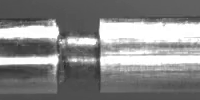
\includegraphics[width=4.9cm, height=3.15cm]{images/copper_f2.png}};
\node[anchor=south west, fill=PSGold, text=black, rounded corners=1.5pt, inner sep=1.2pt] at (35.65, 29.08) {\bfseries\fontsize{6.5}{7.5}\selectfont $35.0\,\mu\text{s}$};
\node[anchor=south east, fill=black!75, text=white, rounded corners=1.5pt, inner sep=1.2pt] at (40.45, 29.08) {\fontsize{6.2}{7.2}\selectfont Elastic};

% Frame 3
\draw[white!40, fill=black, line width=0.6pt] (40.75, 29.0) rectangle (45.75, 32.25);
\node[inner sep=0pt] at (43.25, 30.625) {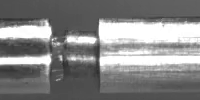
\includegraphics[width=4.9cm, height=3.15cm]{images/copper_f3.png}};
\node[anchor=south west, fill=PSGold, text=black, rounded corners=1.5pt, inner sep=1.2pt] at (40.85, 29.08) {\bfseries\fontsize{6.5}{7.5}\selectfont $70.0\,\mu\text{s}$};
\node[anchor=south east, fill=black!75, text=white, rounded corners=1.5pt, inner sep=1.2pt] at (45.65, 29.08) {\fontsize{6.2}{7.2}\selectfont Flow};

% Frame 4
\draw[white!40, fill=black, line width=0.6pt] (45.95, 29.0) rectangle (50.95, 32.25);
\node[inner sep=0pt] at (48.45, 30.625) {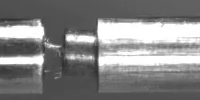
\includegraphics[width=4.9cm, height=3.15cm]{images/copper_f4.png}};
\node[anchor=south west, fill=PSGold, text=black, rounded corners=1.5pt, inner sep=1.2pt] at (46.05, 29.08) {\bfseries\fontsize{6.5}{7.5}\selectfont $105.0\,\mu\text{s}$};
\node[anchor=south east, fill=black!75, text=white, rounded corners=1.5pt, inner sep=1.2pt] at (50.85, 29.08) {\fontsize{6.2}{7.2}\selectfont Barreling};

% Frame 5
\draw[white!40, fill=black, line width=0.6pt] (51.15, 29.0) rectangle (56.15, 32.25);
\node[inner sep=0pt] at (53.65, 30.625) {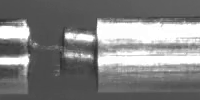
\includegraphics[width=4.9cm, height=3.15cm]{images/copper_f5.png}};
\node[anchor=south west, fill=PSGold, text=black, rounded corners=1.5pt, inner sep=1.2pt] at (51.25, 29.08) {\bfseries\fontsize{6.5}{7.5}\selectfont $140.0\,\mu\text{s}$};
\node[anchor=south east, fill=black!75, text=white, rounded corners=1.5pt, inner sep=1.2pt] at (56.05, 29.08) {\fontsize{6.2}{7.2}\selectfont Perm.\ Set};

% Text under filmstrip
\node[anchor=north west, text width=26.1cm, inner sep=0pt, align=left] at (30.2, 28.2) {%
  \fontsize{10.2}{14.5}\selectfont
  \begin{itemize}\setlength{\itemsep}{0.28em}\setlength{\leftmargin}{1.0em}
    \item \textbf{Deformation Kinematics:} In-situ high-speed sequence captures progressive axial upsetting, uniform radial expansion, and plastic barreling without shear localization.
    \item \textbf{Dynamic Contact \& Interface Uniformity:} Sub-microsecond exposure verifies planar platen seating and absence of specimen tilt or reverberating acoustic reflections during wave entry.
    \item \textbf{Full-Field Optical Strain Tracking:} Synchronous frame recordings enable digital image correlation (DIC) to cross-validate bar 1D wave reduction against true surface kinematics.
  \end{itemize}
};


% ============================================================
% ROW 3 (y = 0.0 to 19.4 cm, h = 19.4 cm):
% Left: Rate-Dependent Response & Failure | Right: Future Horizons (1,000 Tests/Day)
% ============================================================

% --- CARD 5: Rate-Dependent Constitutive Response & Failure Diagnostics ---
\ModernCardHeader{0}{0.0}{27.5}{19.4}{Rate-Dependent Response \& Failure Diagnostics}{Material Behavior}

% Composite Image: PMMA Stress-Strain + SEM Shear Kinking + Micro-CT Scan
\node[anchor=north] at (13.75, 18.0) {%
  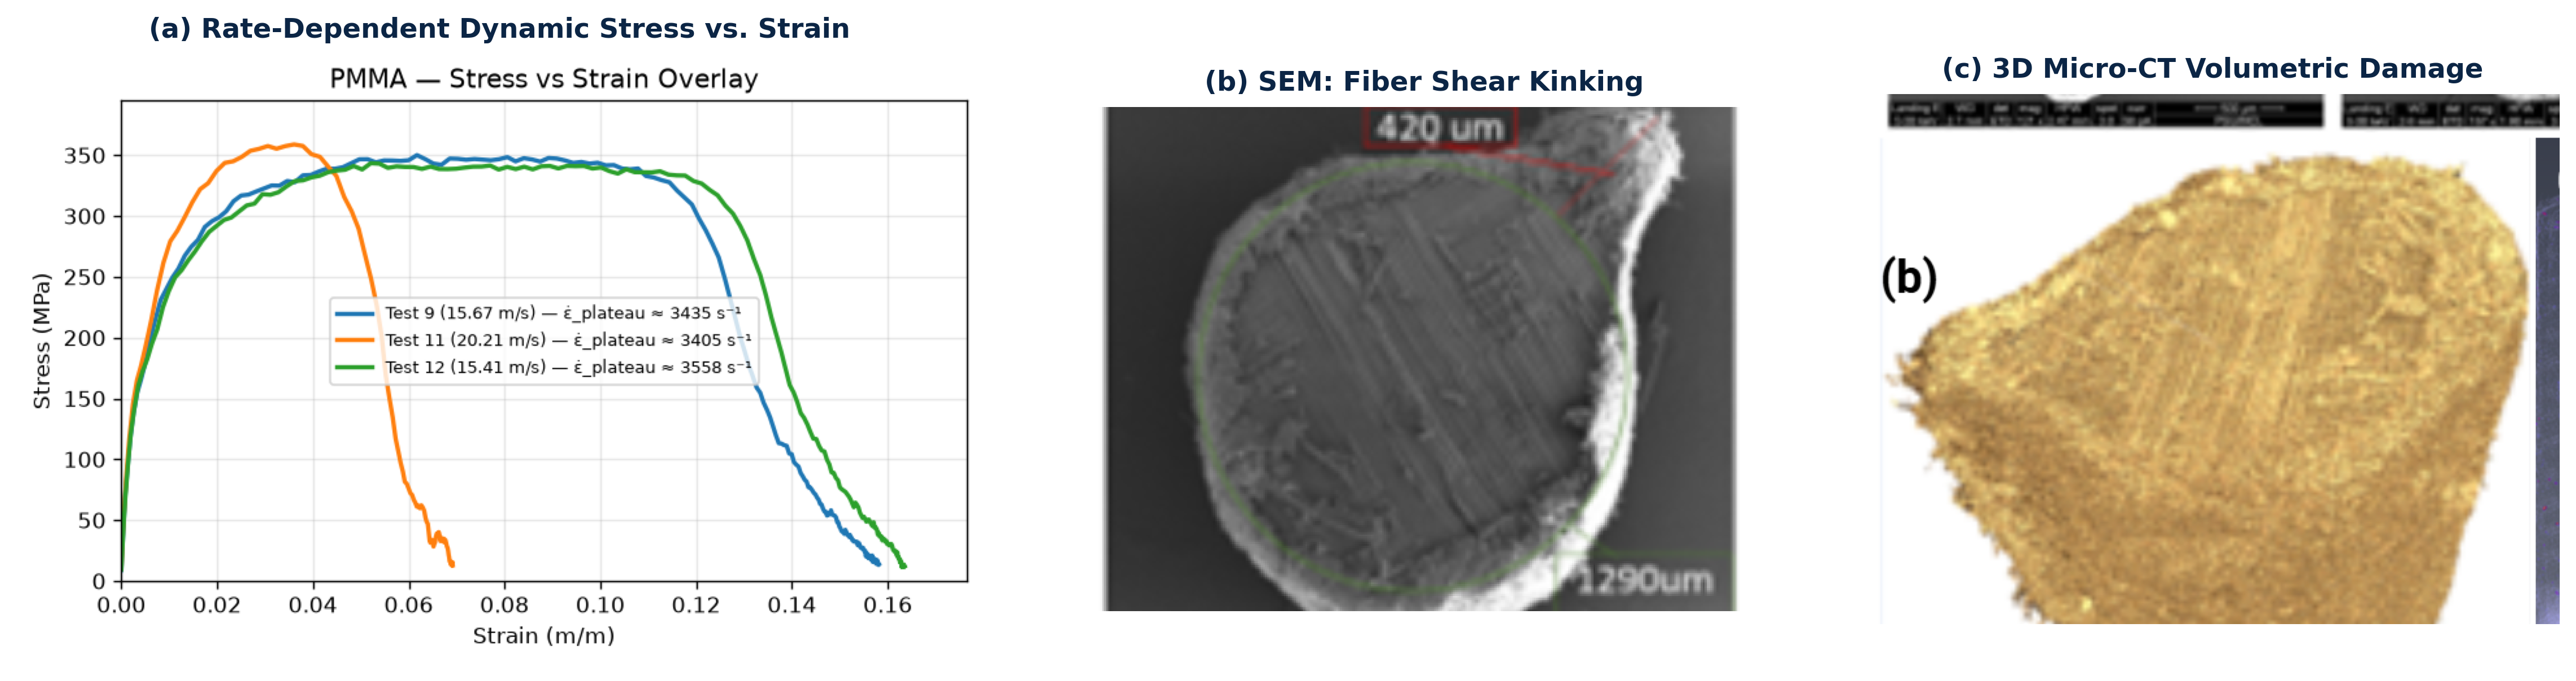
\includegraphics[width=26.2cm, height=7.5cm, keepaspectratio]{images/rate_and_damage_composite.png}%
};

% Text Box for Card 5
\node[anchor=north west, text width=26.1cm, align=left] at (0.7, 10.3) {%
  \fontsize{10.2}{14.5}\selectfont
  \begin{itemize}\setlength{\itemsep}{0.28em}\setlength{\leftmargin}{1.0em}
    \item \textbf{Extended Constant Strain-Rate Plateau:} Tailored pulse shaping yields a flat strain-rate plateau ($\dot{\varepsilon} \approx 3400\text{--}3560\,\text{s}^{-1}$), ensuring constitutive data is uncontaminated by transient wave accelerations.
    \item \textbf{Dynamic Yield \& Flow Enhancement:} PMMA specimens exhibit distinct rate hardening, elevating flow stress to $\sim 345\,\text{MPa}$ at high rates compared to quasi-static yield values ($\sim 100\,\text{MPa}$).
    \item \textbf{Micro-Scale Failure Mechanisms:} Post-test SEM imaging reveals transverse fiber shear kinking, matrix crushing, and dynamic spallation at rates $>10^3\,\text{s}^{-1}$.
    \item \textbf{Symbiotic Digital Twin Feedback:} Experimental flow stress curves and 3D micro-CT damage fields directly inform and calibrate anisotropic plasticity and dynamic failure criteria in LANL penetration simulations.
  \end{itemize}
};


% --- CARD 6: Future Horizons: Autonomous High-Throughput Kolsky Bar ---
\ModernCardHeader{29.5}{0.0}{27.5}{19.4}{Future Horizons: Autonomous Kolsky Bar System}{1,000 Tests / Day}

% Image: High-Throughput Autonomous Workflow Architecture (Robotic Carousel -> Digital Twin Inversion -> Model Discovery)
\node[anchor=north] at (43.25, 18.0) {%
  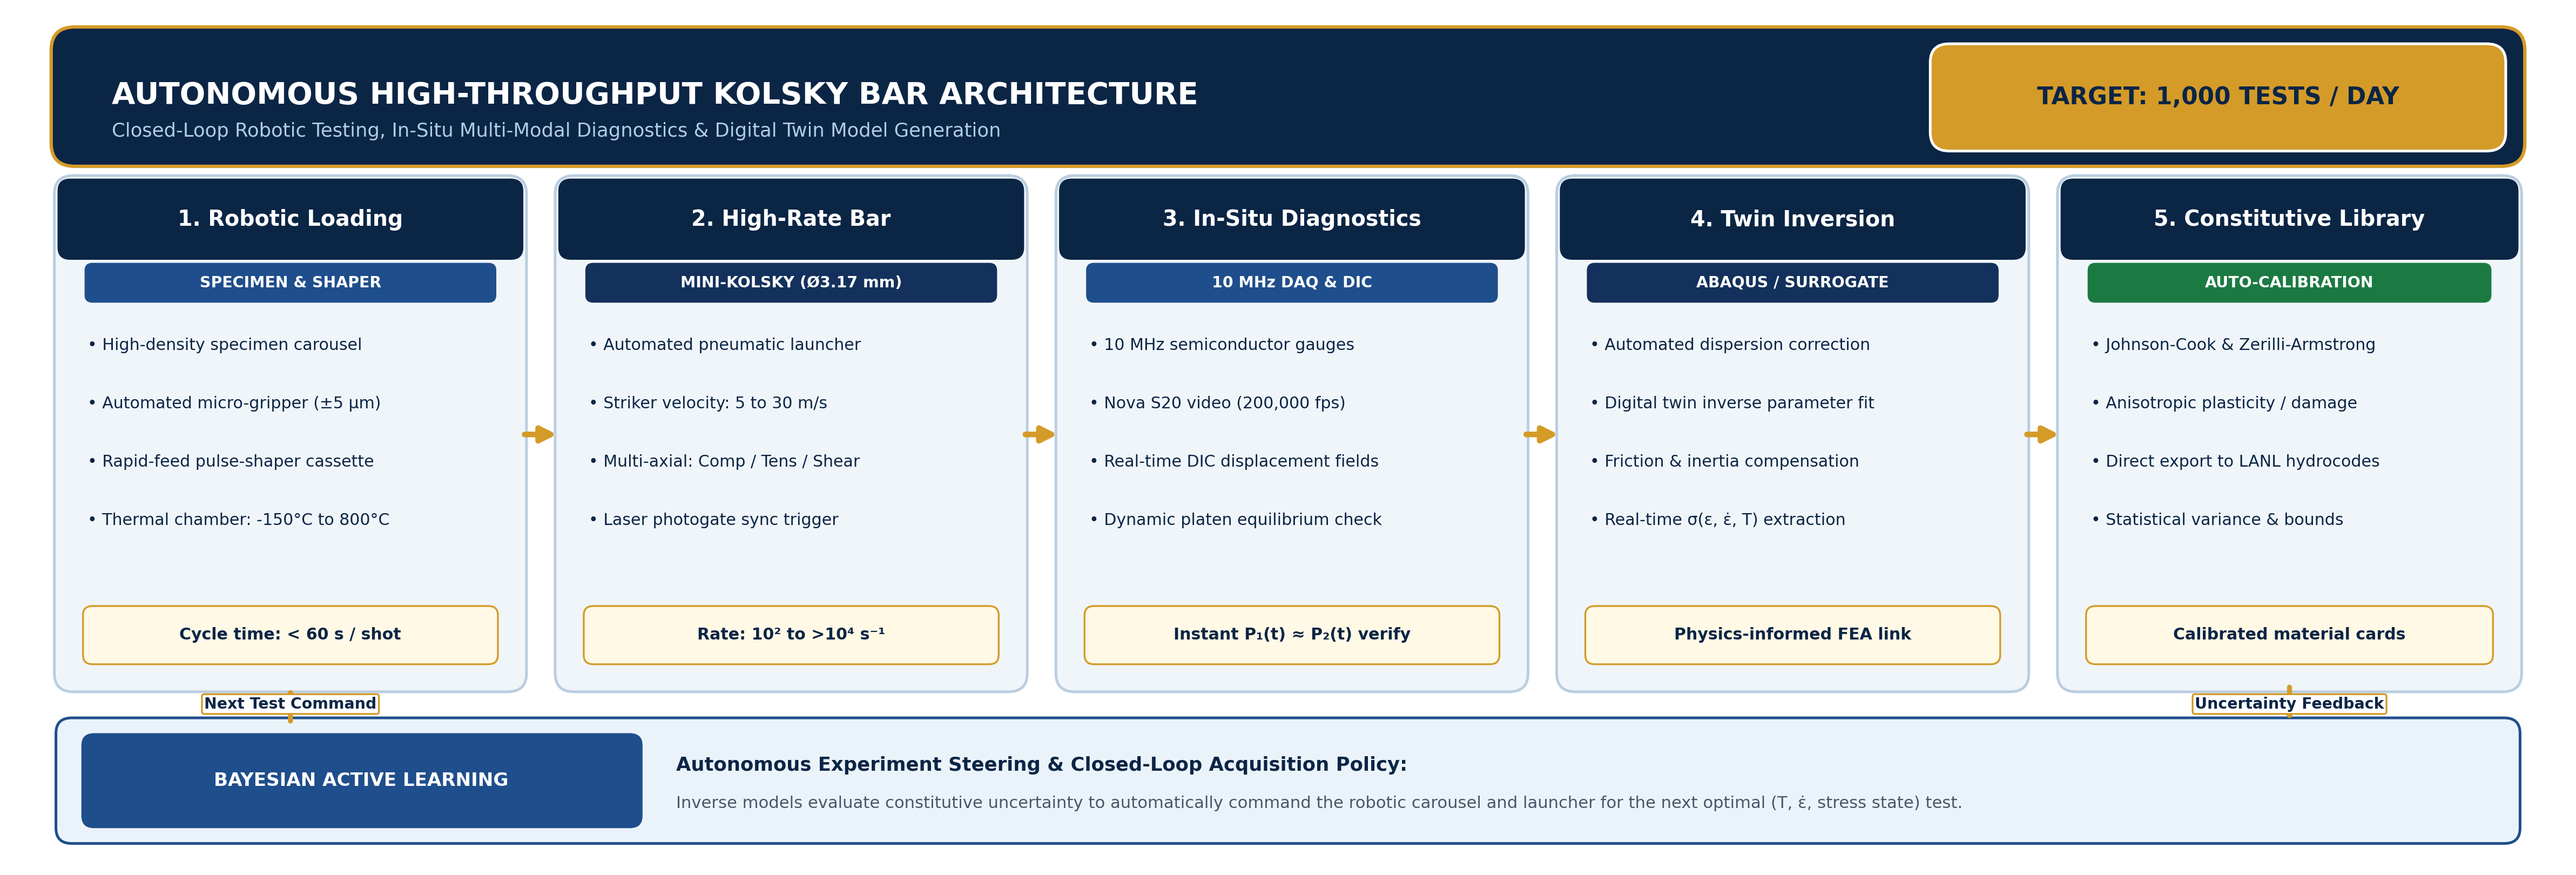
\includegraphics[width=26.2cm, height=8.0cm, keepaspectratio]{images/automation_concept.png}%
};

% Text Box for Card 6
\node[anchor=north west, text width=26.1cm, align=left] at (30.2, 9.8) {%
  \fontsize{10.2}{14.5}\selectfont
  \begin{itemize}\setlength{\itemsep}{0.28em}\setlength{\leftmargin}{1.0em}
    \item \textbf{Autonomous 1,000-Tests/Day Throughput:} High-density robotic carousels, automated pick-and-place micro-grippers ($\pm 5\,\mu\text{m}$), and rapid-cycle pulse-shaper cassettes achieve $<60\,\text{s}$ shot turnaround.
    \item \textbf{Multi-Condition Parametric Testing:} Rapid automated sweeps across wide thermal bounds ($-150^\circ\text{C}\text{ to }800^\circ\text{C}$), strain rates ($10^2\text{--}10^4\,\text{s}^{-1}$), and multi-axial stress states (compression, shear, tension).
    \item \textbf{Active Learning Experiment Steering:} Bayesian acquisition algorithms identify high-uncertainty regions in constitutive space, automatically commanding the next test conditions to maximize information gain.
    \item \textbf{Automated Rate-Dependent Model Discovery:} Synchronized $10\,\text{MHz}$ DAQ and DIC feed into automated inverse FE solvers, auto-calibrating Johnson-Cook and damage models for direct LANL hydrocode deployment.
  \end{itemize}
};

\end{scope}
\end{tikzpicture}

\end{document}